% This is samplepaper.tex, a sample chapter demonstrating the
% LLNCS macro package for Springer Computer Science proceedings;
% Version 2.20 of 2017/10/04
%
\documentclass[runningheads]{llncs}
%
\usepackage{graphicx}
\usepackage{xcolor}
\usepackage{todonotes}
\usepackage{listings,xcolor}
\colorlet{punct}{red!60!black}
\definecolor{background}{HTML}{EEEEEE}
\definecolor{delim}{RGB}{20,105,176}
\colorlet{numb}{magenta!60!black}

\lstdefinelanguage{json}{
	basicstyle=\normalfont\ttfamily,
	numbers=left,
	numberstyle=\scriptsize,
	stepnumber=1,
	numbersep=7pt,
	showstringspaces=false,
	breaklines=true,
	frame=lines,
	%backgroundcolor=\color{background},
	literate=
	*{0}{{{\color{numb}0}}}{1}
	{1}{{{\color{numb}1}}}{1}
	{2}{{{\color{numb}2}}}{1}
	{3}{{{\color{numb}3}}}{1}
	{4}{{{\color{numb}4}}}{1}
	{5}{{{\color{numb}5}}}{1}
	{6}{{{\color{numb}6}}}{1}
	{7}{{{\color{numb}7}}}{1}
	{8}{{{\color{numb}8}}}{1}
	{9}{{{\color{numb}9}}}{1}
	%{:}{{{\color{punct}{:}}}}{1}
	%{,}{{{\color{punct}{,}}}}{1}
	{\{}{{{\color{delim}{\{}}}}{1}
	{\}}{{{\color{delim}{\}}}}}{1}
	{[}{{{\color{delim}{[}}}}{1}
	{]}{{{\color{delim}{]}}}}{1},
}

\newcommand{\rtodo}[1]{\textcolor{red}{#1}}

\begin{document}
	%
	\title{CrOwS - Crowd Overwatch System}
	
	\author{Group 2: Felix Bühler \and
		Jan Leusmann \and
		Jamie Ullerich}
	
	\institute{Service Computing Department, IAAS, University of Stuttgart \\ https://github.com/Stunkymonkey/Iot-university
		%\email{firstname.lastname@uni-stuttgart.de}
	}
	%
	\maketitle              % typeset the header of the contribution
	%
	\begin{abstract}
		%The abstract should briefly summarize the contents of the report in
		%150--250 words. 
		Due to the current ongoing COVID-19 pandemic, many daily tasks come with the risk of becoming infected or infecting others.
		We have built a smart supermarket, which should minimize the risk of being infected with the corona virus.
		Since it can be dangerous to be in large crowds, it is important to limit the number of people in the supermarket and at the same time keep waiting times to a minimum for comfort.
		Furthermore, the employees should be protected as well as possible and a good air quality must be ensured. 
		While current markets have rather improvised solutions, a smart building that protects the privacy of the customer would be better to not only increase safety for customers but also employees. 
		Therefore, we have built a prototype that helps to handle the requirements more easily. 
		In this work, we describe how our system is constructed, which requirements are fulfilled and how this was implemented.  
		\keywords{Smart Building \and Internet of Things}
	\end{abstract}
	%
	%
	%
	\section{System Introduction}
	%Describe the scope (background information and problem statement) and the goals of your project.
	%Table~\ref{tab1} an example of a table.
	%\begin{table}
	%\caption{Table captions should be placed above the tables.}\label{tab1}
	%\begin{tabular}{|l|l|}
	%\hline
	%Item & Deadline \\
	%\hline
	%I1 & D1 \\
	%\hline
	%\end{tabular}
	%\end{table}
	%Fig.~\ref{fig1} gives an example of a figure.
	
	%\begin{figure}
	%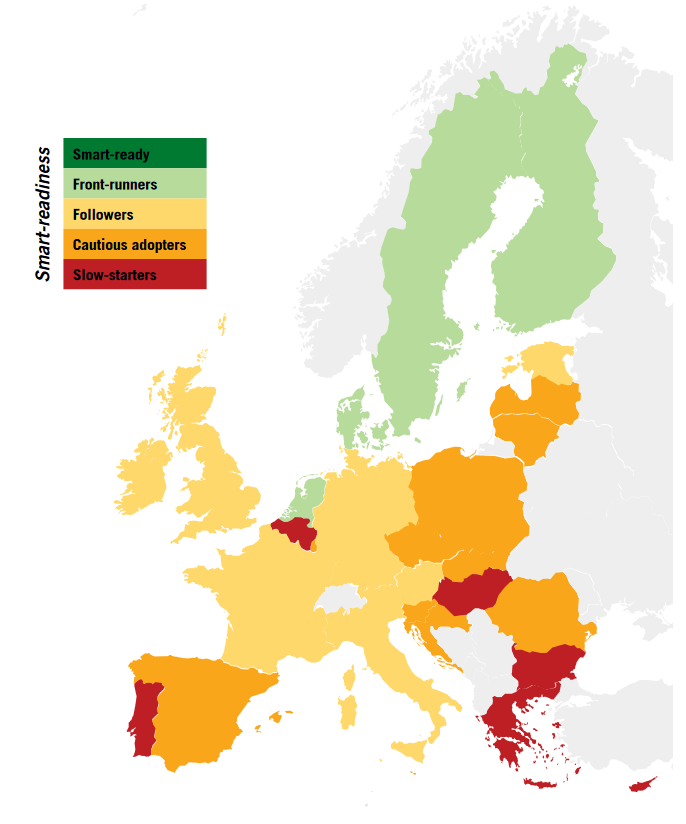
\includegraphics[width=\textwidth]{fig1}
	%\caption{A figure caption is always placed below the illustration. Please note that short captions are centered, while long ones are justified by the macro package automatically.} \label{fig1}
	%\end{figure}
	
	%For citations of references, we prefer the use of square brackets and consecutive numbers. The following bibliography provides a sample reference list with entries for journal articles~\cite{ref_article1}, a book~\cite{ref_book1}, proceedings without editors~\cite{ref_proc1}, and a homepage~\cite{ref_url1}. Multiple citations are grouped \cite{ref_article1,ref_book1}, \cite{ref_article1,ref_book1,ref_proc1,ref_url1}.
	Since the outbreak of the corona virus social distancing has become the norm and leaving the house should be done only for necessary tasks.
	Shopping for groceries is a mandatory task and to decrease the risk of infection, the number of people inside a public building is regulated.
	Currently this regulation is mostly done by employees, who count how many people are inside the supermarket.
	This poses different problems.
	First, the employee who counts entering people has to interact with every customer and puts himself at a greater risk of becoming infected. 
	Also, humans are prone to make mistakes.
	This is why we chose to build a smart supermarket in this project.
	\\ \linebreak
	An automated system could improve this task by having detailed information about the state of the supermarket and automating tasks, like counting people entering and leaving the supermarket.
	The state should consist of knowledge about the number of people, as well as the state of the air quality and the amount of remaining purchasable goods.
	To have a more fine granular view of this state we also wanted to divide the supermarket into subsections.
	This does make sense in a real world scenario, as this leads to people not potentially infecting every person in the supermarket, but only the ones who shop the same type of groceries as themselves. 
	Also this decreases the risks of infecting employees, who have to refill shelves, as the system has knowledge about the state of shelves and amount of people inside a section. 
	Employees will be notified when a shelf is empty, but they are only allowed to enter the section to refill the shelf when the number of people inside this section is low. 
	This makes the system not only useful during the time of the pandemic, but could also help supermarkets in a more general way.
	One wonted problem when shopping for groceries are clusters of customers in front of specific shelves. 
	Our system is able to tackle this problem, by assigning each subsection of the supermarket a limited number of people who are allowed to be in the subsection at the same time. 
	Also closing subsections when the shelves are empty makes it easier for employees to refill goods, as they do not have to wait for customers to move out of the way.
	\\ \linebreak
	One further goal we had for this project was to make the implementation modular such that we could always extent the system with additional sensors and actuators. 
	This is why we chose to have a single file for each system component, which would send or receive data needed for this component. 
	This does not only ensure modularity, but also enables the possibility to have components run on different devices without problem.
	\\ \linebreak
	All in all our system is able to decrease the risk of infection when shopping for groceries, to increase productivity for employees, and to decrease waiting times for customers.
	The resulting smart supermarket was built mostly with parts we already owned, which is why some design choices were made in order to make use of the parts we had available.
	However, smart buildings can have many more functions which we did not include in our project. 
	This is especially important for non-residential buildings like supermarkets, since those kinds of buildings are used by lots of people and it is possible to automate various tasks.
	Further advantages of smart buildings in this area include saving energy, a greater safety for users and a more convenient shopping experience. 
	This is why building such smart supermarkets will be important in the future and should already be put into practice in order to become a natural part of our everyday life. 
	In the following report about our system we first do a system analysis, then talk about the system architecture design, explain the system implementation, and lastly discuss limitations and problems of the system. 
	
	\section{System Analysis}
	%Describe the user requirements of your system.
	We identified 13 system requirements, which are listed and discussed below. 
	This is followed by the description of a use case, which uses an example to show how the system works.
	\begin{figure}[h!]
		\centering
		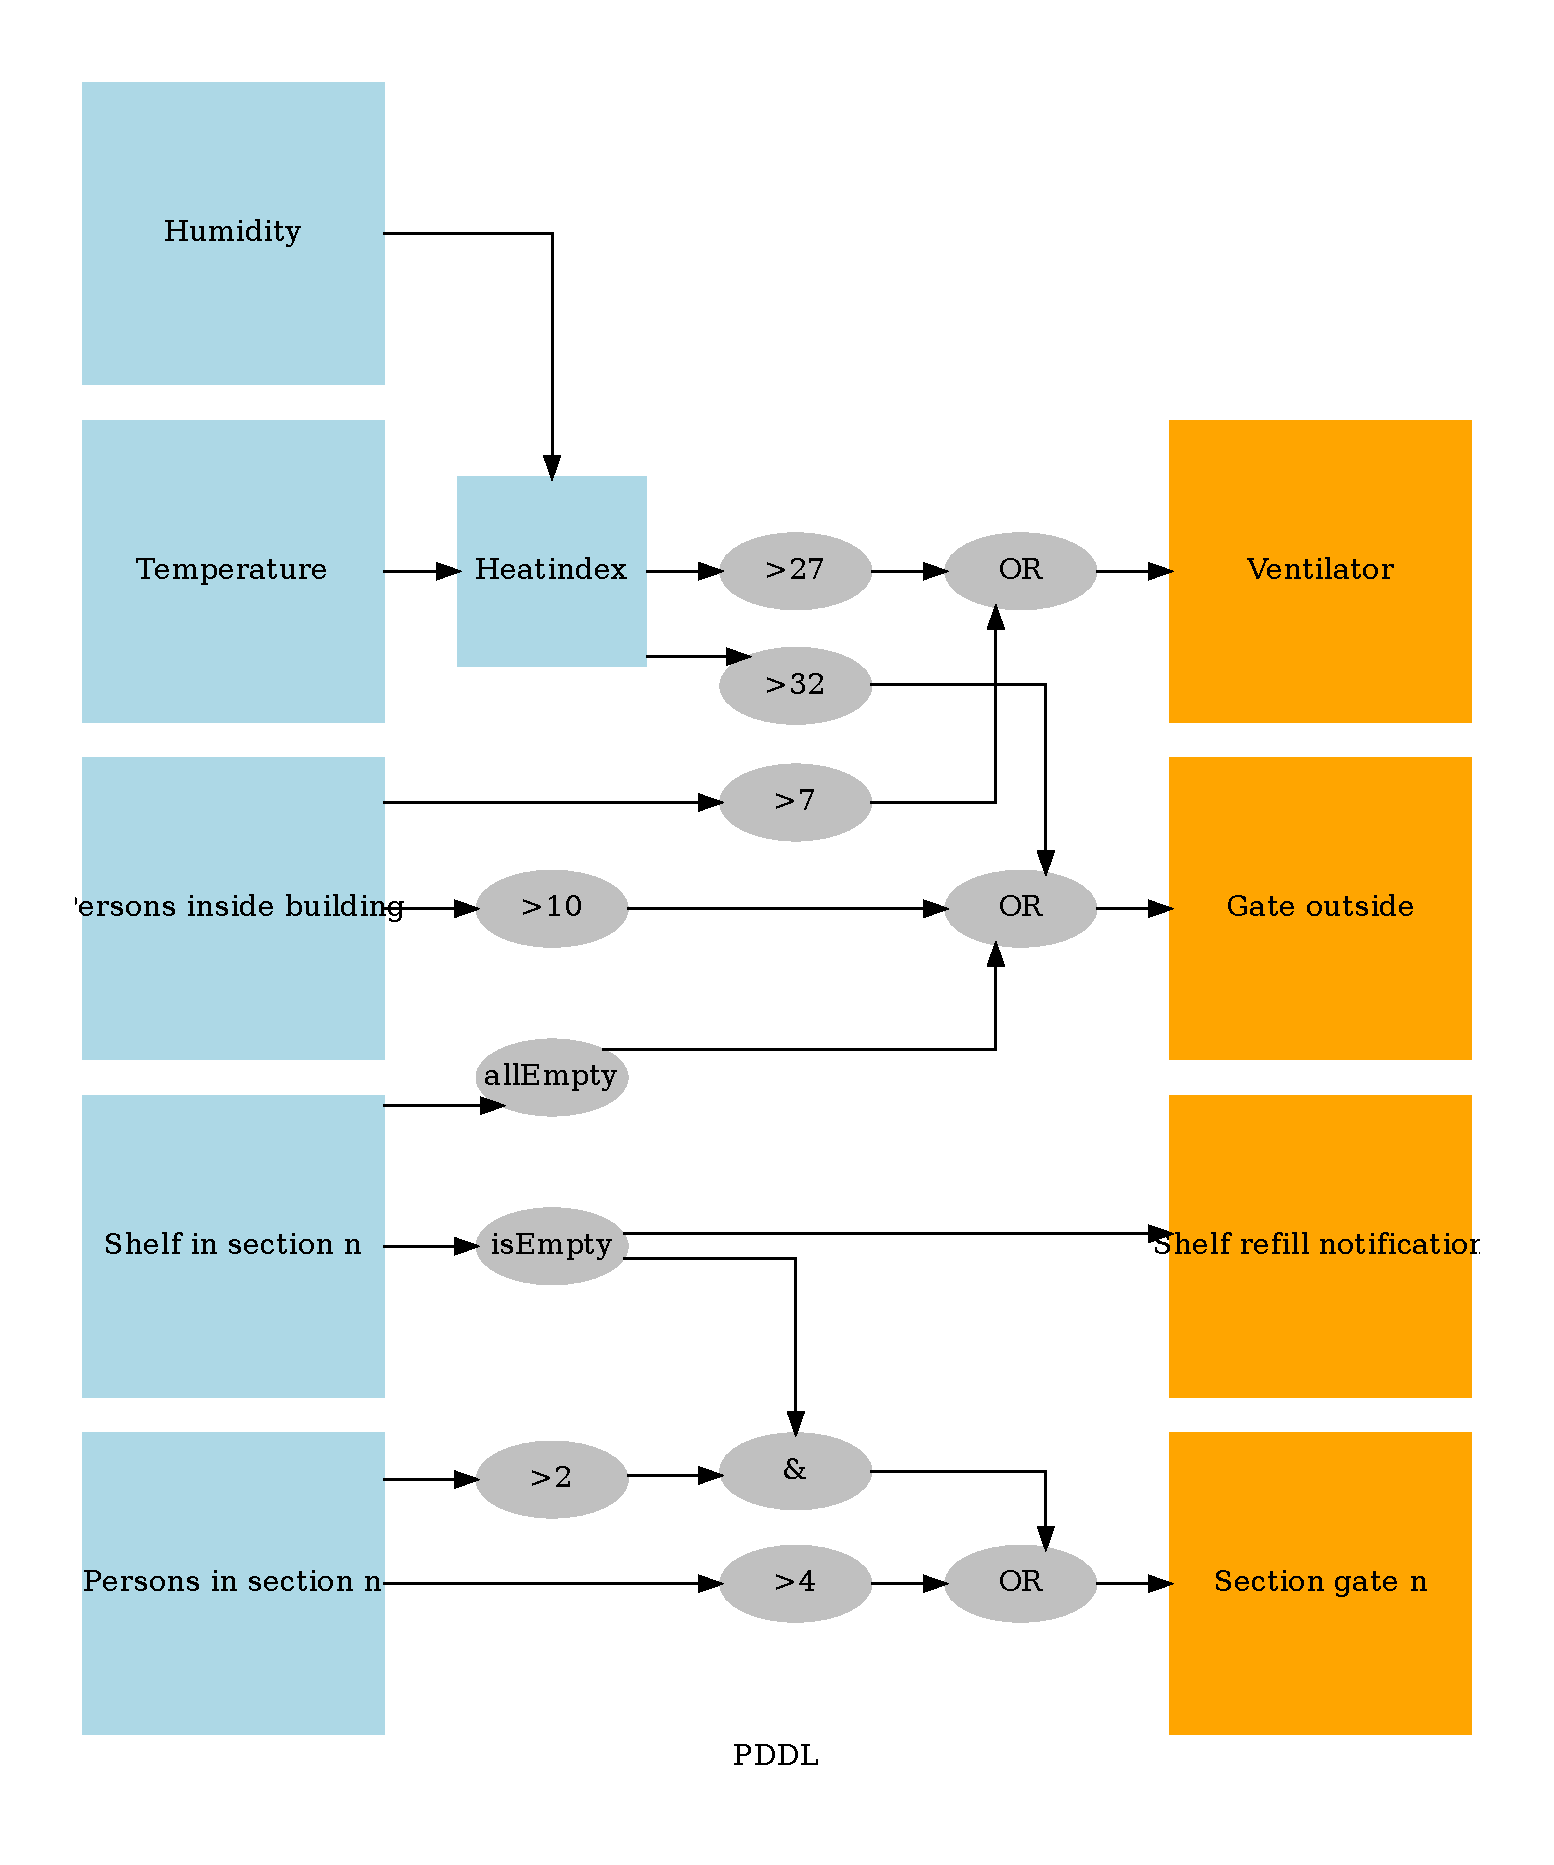
\includegraphics[width=\linewidth]{figures/decision_tree.pdf}
		\caption{This graph shows how the system uses sensor values to decide which command the corresponding actuator should execute.}
		\label{fig:decision}
	\end{figure}
	\clearpage
	\subsection{System Requirements}
	As functional requirements, the system should: 
	\begin{enumerate}
		\item sense temperature and humidity 
		\item know the amount of people in each section
		\item use this information to decide when to improve the air quality by turning on a ventilator
		\item prohibit people from entering a section if there is no more space
		\item prohibit people from entering a section if the shelf is empty and too many people are already inside
		\item prohibit people from entering the supermarket if the heat index is too high
		\item prohibit people from entering the supermarket if there are too many people inside
		\item prohibit people from entering the supermarket if all shelves are empty 
		\item monitor the filling level of the shelves 
		\item send notifications to workers if a shelf needs refilling 
	\end{enumerate}
	Non-functional requirements demand that the system: 
	\begin{enumerate}
		\item does not invade people's privacy 
		\item keeps the involvement of the users minimal 
		\item is scalable in case new sections are added
	\end{enumerate}
	The components, which fulfil the functional requirements are described in section~\ref{sec:architecture}. 
	Regarding the non-functional requirements, our system preserves the privacy of the users, since we do not collect any data other than how many people are inside (non-functional requirement 1).
	The user is little involved since he only needs to press a button when leaving or entering a section (non-functional requirement 2).
	However, this could be minimised by using other tracking techniques, such as a video camera to collect information about where people are. 
	But this would then lead to collecting more information about the users and therefore invade their privacy more. 
	This trade-off between comfort and privacy should be considered. 
	The last non-functional requirement demands a scalable system (non-functional requirement 3).
	Our system can be easily extended with more sections since most components of our system are loosely coupled. 
	This is important because our system should fit into as many different markets as possible and it should still work after a restructuring of the supermarket too.
	\begin{figure}[bt]
		\centering
		\includegraphics[width=\linewidth]{figures/floorplan1.pdf}
		\caption{The floor plan of our supermarket, including an exemplary arrangement of perople.}
		\label{fig:floorplan}
	\end{figure}
	\subsection{Use case scenario}
	This use case demonstrates the system's functionality and is illustrated simplified in Figure~\ref{fig:floorplan}.
	The rules on which the system acts on are shown in Figure~\ref{fig:decision}, as well.
	Since there are currently five people in section 1, the system must prohibit more people from entering by showing it on the LED Matrix outside. 
	This is important for the safety of the customers, since a minimum distance must always be maintained to reduce the risk of becoming infected. 
	A lot of people take items from the shelf, indicating that it must be refilled soon. 
	This will be confirmed by the proximity sensor. 
	The system must send a notification to the worker and keep the do-not-enter-sign to ensure there are little enough people in the room that the worker can safely restock the shelf.
	As there is only one person in section 2, the LED Matrix will show the number one. 
	This must be changed when the person which is about to leave presses the button. 
	Since there are a lot of people in the supermarket and the temperature and humidity sensor will most likely report a value which exceeds the thresholds, the system will then turn on the ventilator to ensure an appropriate air quality is maintained. 
	If the threshold is far exceeded, the system should not let any more people into the building until the heat index returned to a safe value.
	Since the air quality decreases when many people are in the same place, which leads to a higher risk of being infected, the fan will be turned on as soon as there are eight people inside. 
	This helps to keep the air permanently fresh. 
	There is still room in the supermarket, which is why the LED outside will be green, indicating that people can still enter.
	In general, the red LED will be switched on if there are more than ten people inside, or if all shelves are empty, as well. 
	The latter case prevents a large number of customers from queuing in a small space and the worker from facing an increased risk of becoming infected.
	
	\section{System Architecture Design}
	%Describe and provide a design of the architecture of your system.
	\label{sec:architecture}
	In this section, we describe the design of the architecture of our system which can be seen in Figure~\ref{fig:architecture}.
	This part is divided into further paragraphs that each describe one respective layer of our architecture. 
	\\ \linebreak
	\begin{figure}[bt]
		\centering
		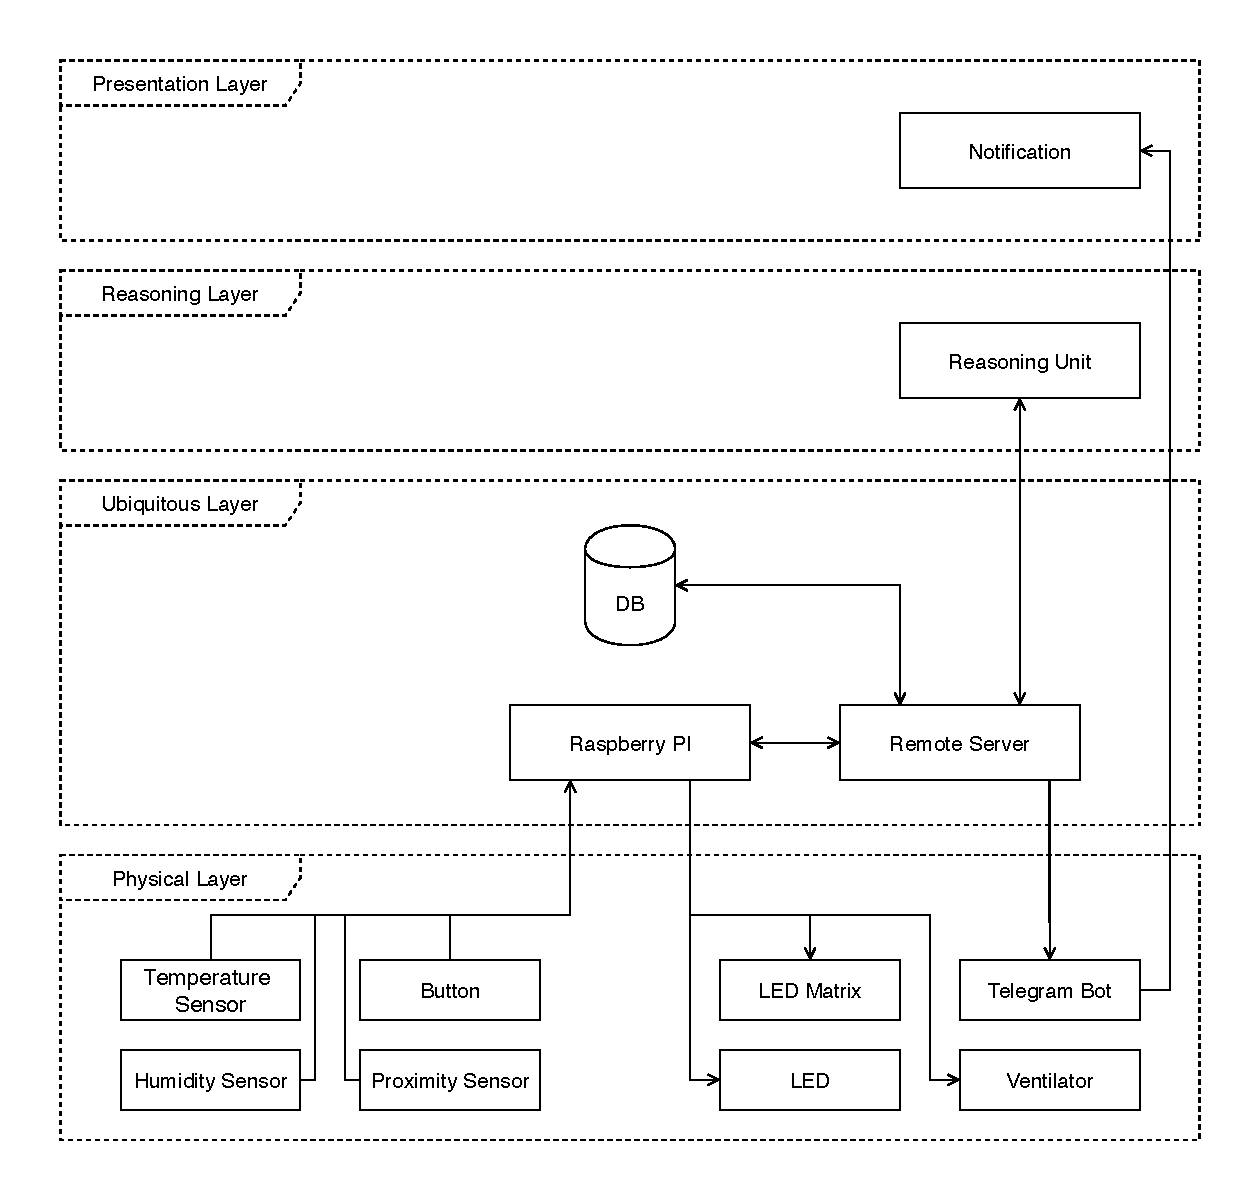
\includegraphics[width=\linewidth]{figures/architecture.pdf}
		\caption{The architecture of our system, showing all components in their corresponding layer.}
		\label{fig:architecture}
	\end{figure}
	\newpage \noindent The physical layer consists of sensors and actuators.
	The former are a temperature and humidity sensor (functional requirement 1), buttons which are used to count the number of people inside each section (functional requirement 2) and proximity sensors which monitor the filling levels of the shelves (functional requirement 5). 
	These sensors are sending information to the Raspberry PI in the next layer, which processes the information. 
	The task of those components is to know the state of the supermarket. 
	In our system, this consists of the air quality, filling levels of the shelves and the number of people in each section. 
	Actuators are LEDs and LED Matrices, showing how many people are inside and if entering is prohibited (functional requirement 4 - 8).
	The task of these components is to provide information to the people inside and outside of the supermarket. 
	In this way, the customers can decide which section to visit first and they know when to wait.
	Additionally, this ensures the safety of people inside the supermarket.
	Another actuator is a ventilator which can be turned on to improve the air quality (functional requirement 3).
	This functionality should not only be used when the quality is poor, but also as a preventive measure. 
	Therefore, the reasoning unit should decide when this task must be executed without delay. 
	The last actuator is the telegram bot~\cite{telegram}. 
	The task of this component is to inform the employee when a shelf must be refilled. 
	This decision will also be obtained from the reasoning unit.
	\\ \linebreak
	The ubiquitous layer contains a raspberry PI, which collects the information reported by sensors and passes instructions to the actuators. 
	The task of this component is the communication of sensors, actuators and the server which processes the information, generates intelligence based on it and then passes the information to the reasoning unit.
	If any state should be changed, it forwards those decisions on how to act next. 
	The server also hosts an emulator which can be used to simulate the values of the sensors and actuators. 
	It is connected to a database which stores all values of sensors and actuators, as well.
	\\ \linebreak
	The reasoning unit in the third layer uses the information provided by the previous parts to decide how to act (functional requirement 3 and 4). 
	The decisions are based on a solution found by using AI-planning. 
	The security of people is very important; therefore, we defined several goals to ensure a minimal infection risk, which are tasks of the reasoning unit. 
	First, as mentioned above, the air quality should be kept good. 
	Therefore, the reasoning unit should take temperature, humidity and the number of people in the supermarket into account for deciding whether to turn on the ventilator. 
	Secondly, the number of people in one room should be minimal, hence the decision whether to close a gate should be based on the number of persons, heat index and filling level of the shelves. 
	Lastly, the shelves should be refilled when empty, while the number of persons in the corresponding section should be kept as low as possible. \\ \linebreak
	The last layer is the presentation layer.
	It contains the notifications, which are presented to the user. 
	In this case, the user is the employee of the supermarket, and receives the message saying which shelf must be refilled (functional requirement 6). 
	
	\begin{figure}
		\centering
		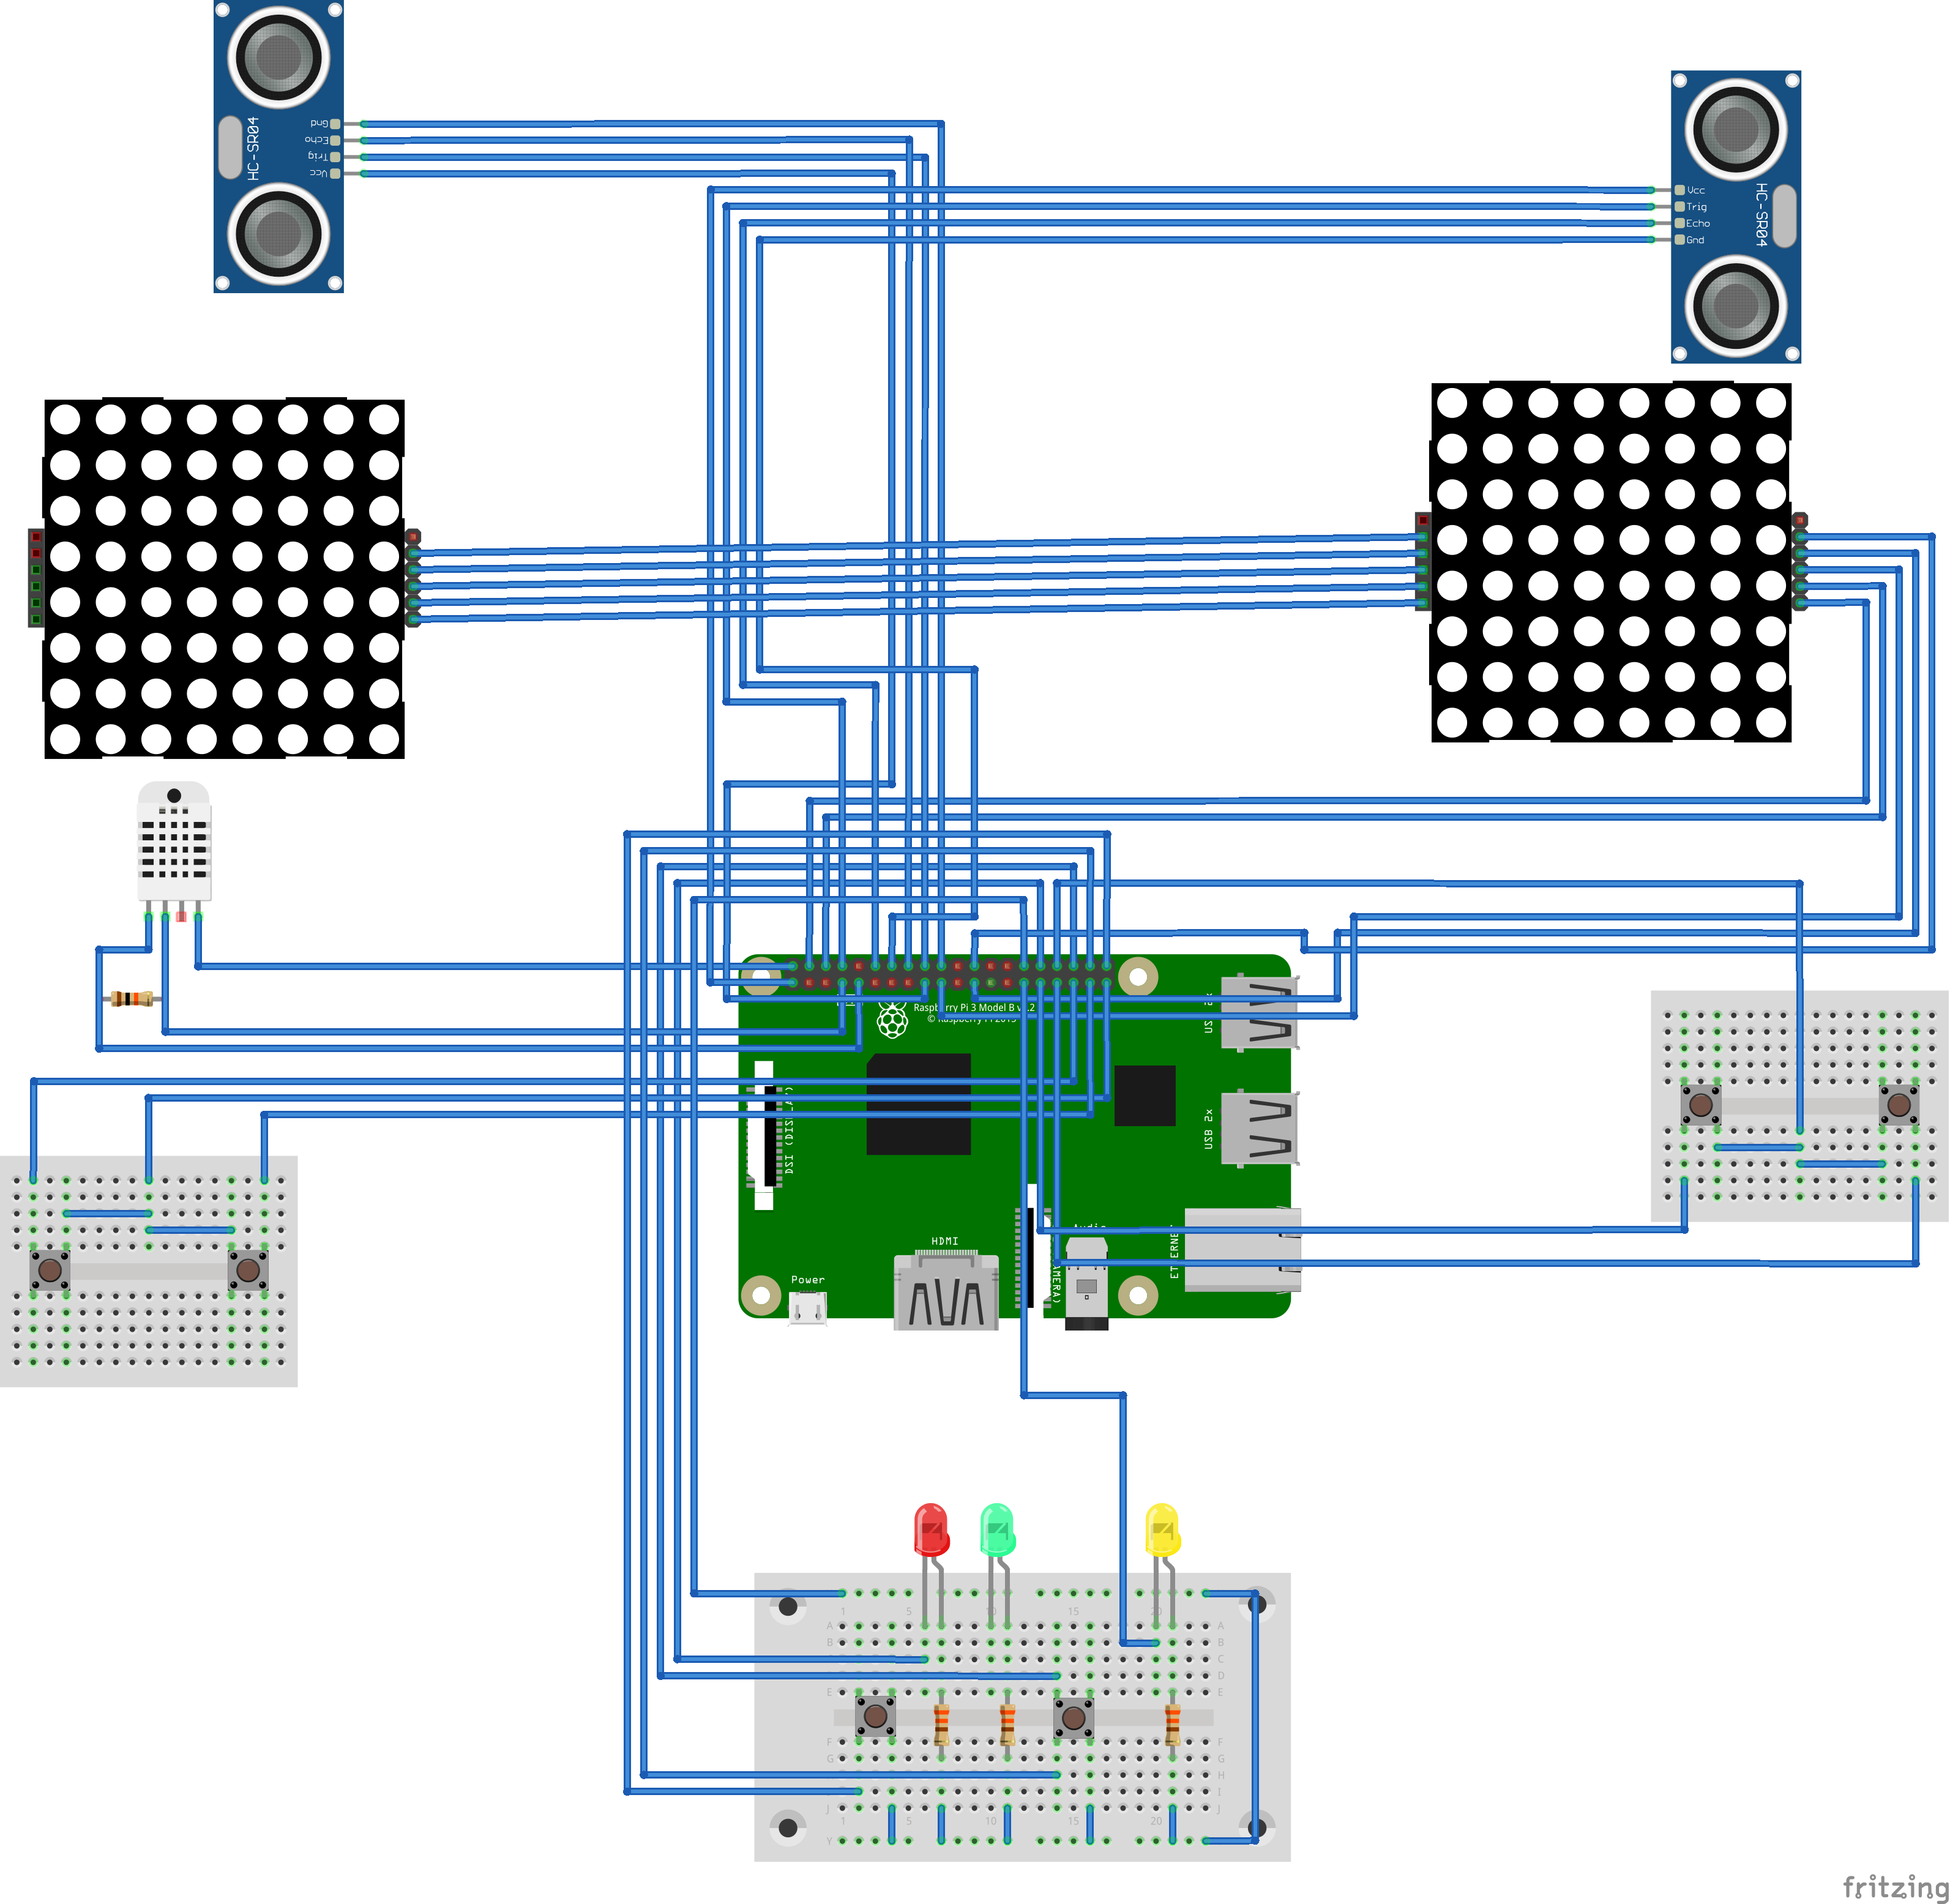
\includegraphics[width=7.5cm]{figures/setup_bb.png}
		\caption{The wiring of our prototype including all sensors and actuators controlled by the Raspberry PI.}
		\label{fig:wiring}
	\end{figure}
	\begin{figure}[bt]
		\centering
		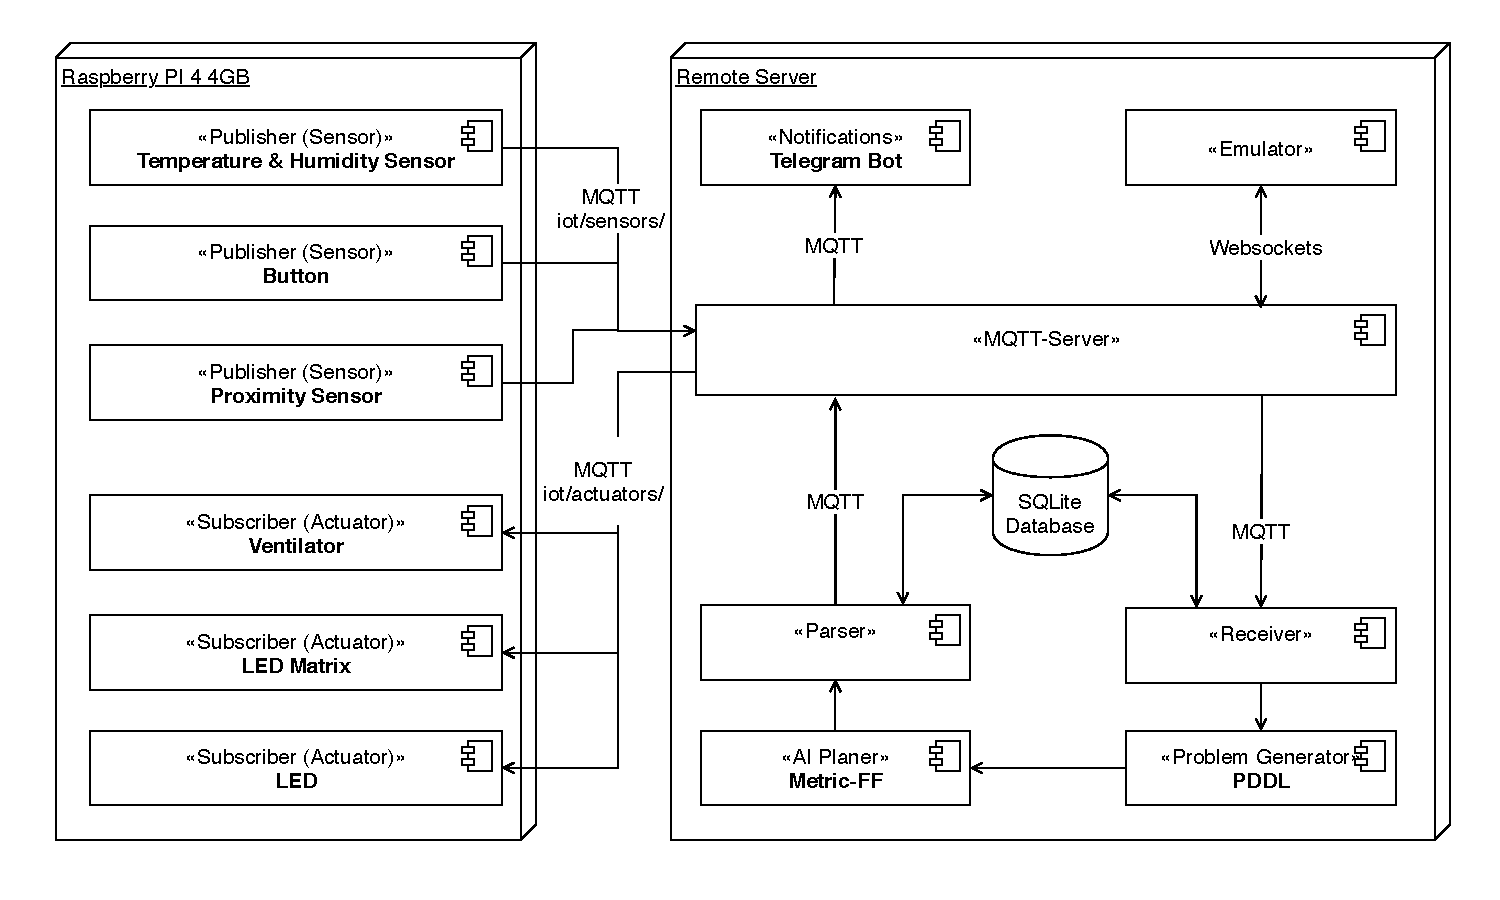
\includegraphics[width=\linewidth]{figures/Deployment.pdf}
		\caption{The setup of our system showing implementation details.}
		\label{fig:setup}
	\end{figure}
	
	\section{System Implementation}
	\label{sec:implementation}
	The following part contains a specification of the used hardware, as well as a detailed description of how our system is implemented. 
	The wiring of the system is depicted in Figure~\ref{fig:wiring}, the concrete setup of our system can be seen in Figure~\ref{fig:setup}.
	\\ \linebreak
	The hardware we use consists of a Raspberry PI 4 - 4GB, the DHT11 temperature and humidity sensor, two HC-SR04+ proximity sensors, two MAX7219 LED Dot Matrices and six IM206 buttons. 
	We used two additional libraries (the proximity sensor~\cite{led-matrix} and the temperature sensor~\cite{dht11}) for accessing the sensors via python.
	The rest was all implemented using the native GPIO-library which is preinstalled on the Raspberry Pi.
	Our used yellow LED is the YF0993-02, green LED is GF0993-02 and the red LED RF0993-02. For displaying the employee notification, we used an Apple iPad to receive the messages from the telegram~\cite{telegram} bot, but this can be replaced by any device on which telegram can be used. 
	\\ \linebreak
	All our components are communicating over MQTT via our own mosquitto-MQTT-Server~\cite{mosquitto}. 
	We hosted it on ``leusmann.io" which runs on an uberspace.de-server with MQTT on port 46980 and websocket on port 46801.
	Our emulator is communicating with MQTT via websockets, this was done because websites can only communicate externally via http. 
	The rest of our components are using MQTT directly. 
	\\ \linebreak
	One main goal was to make the sensor and actuator system as modular as possible. 
	This is achieved by separating every sensor and actuator into a separate file to provide maximum flexibility. 
	Each of the components could be hosted on a separate device if needed. 
	In our case we use the Raspberry Pi for all sensors and actuators except the telegram bot~\cite{telegram}. 
	\\ \linebreak
	In MQTT we divided the sensors and actuators in two different topics according to their purpose. 
	For example, the proximity sensor was publishing on the following topic: ``iot/sensors/section1/shelf" which could activate the telegram bot via  ``iot/actuators/section1/refill\_shelf". 
	The complete topic structure can be seen in Listing~\ref{lst:structure}, where section 0 represents the entrance area of our supermarket.
	\\ \linebreak
	For the AI-planning part, we used the Metric-FF~\cite{ff} planer since it supports numeric fluents.
	Our PDDL domain file contains functions for the number of people, heat index and the number of shelf items. 
	In this way, we can use numerical constraints to ensure that the values are in our defined interval. 
	We defined an action to turn on the ventilator, refill shelves, close sections and close the gate of the supermarket. 
	Our goals respectively demand that the heat index, number of people in each section and the supermarket are below our threshold and the shelves should always be not empty. 
	The decisions are based on Figure~\ref{fig:decision}, as described above. 
	\\ \linebreak
	The temperature and proximity sensor are publishing every few seconds if there is a new measurement. 
	All sensor values are sent raw over MQTT and are not getting interpreted. 
	On the other end there is a receiving python-script running. It takes all sensor values and places them in the database into a separate sensor-table. 
	Our database acts as a key-value storage.
	We use the supported ``UPSERT" to update or insert new unknown values.
	After this it crawls values from the sensor table and exports it into our problem file for the AI-planning. 
	Then the Metric-FF~\cite{ff} planner is used to decide which actuators should be on or off. 
	We input our calculated heat index, the number of items in the shelf and the number of people in each section. 
	The output of the Metric-FF~\cite{ff} is then parsed, and we search for which steps to do. 
	If one step matches our predefined pattern, then the actuator is activated. 
	In our case activating the gate means closing it. %\\ \linebreak
	\begin{lstlisting}[language=json,firstnumber=1,caption={The used MQTT topic structure.},captionpos=b,label={lst:structure}]
	{"iot": {
	"sensor": {
	"section0":{
	"temperature": 27.0,
	"humdity": 40.0,
	"button": {
	"in": 0,
	"out": 0
	}
	},
	"section1":{
	"shelf": 3.5,
	"button": {
	"in": 0,
	"out": 0
	}
	},
	"section2":{
	"shelf": 16.1,
	"button": {
	"in": 0,
	"out": 0
	}
	}
	},
	"actuators":{
	"section0":{
	"gate": "False",
	"ventilator": "True"
	},
	"section1":{
	"gate": "False",
	"refill_shelf": "False"
	},
	"section2":{
	"gate": "True",
	"refill_shelf": "True"
	}
	}
	}
	}
	\end{lstlisting}
	The result of this is then compared to the actuator-table in our database. 
	If the value is the same, then no messages are sent. 
	If the values are different, then the new value is written to the database and a MQTT-message is sent to the actuators.
	\\ \linebreak
	We also implemented an emulator, in which all sensor values can be modified and all actuator outputs can be seen directly. 
	The emulator can run at the same time as the rest of our implementation as it simply acts as an additional physical layer, but simulated. 
	It creates and pushes sensor values and reads incoming actuator values. 
	The emulator was written in vue.js \cite{vue} and we used the vue-mqtt \cite{vue-mqtt} package for MQTT implementation.
	
	
	\section{Discussion and Conclusions}
	%Here you can discuss some interesting points or limitations of your system and conclude the report.
	In this section, we describe some limitations of our project and how they could be improved. 
	It is then concluded with a short summary. 
	\\ \linebreak
	Sadly, one of our proximity sensors broke due to being wrongly connected by mixing up VCC and GND. 
	Since we developed an emulator this was not a big issue, but it is not ideal for demonstration purposes.
	\\ \linebreak
	One limitation of our system is that our temperature/humidity and proximity sensors do not have an internal state and only send an update if something new happens.
	Changing this would reduce the bandwidth, but due to the measurement noise of the sensors, this is not very helpful. 
	One approach could be to only send and save a new value if there is a change by a certain threshold. 
	Another approach would be to use a ``DHT22" sensor for temperature and humidity because it is much more accurate and hence the heat index will have less noise and will be more precise. 
	We think a combination of both would be the best for precision and bandwidth. 
	The same applies for the proximity sensor by using a ``Maxbotix HRLV-EZ1" sensor. 
	\\ \linebreak
	Our sensors are designed to be very modular and each sensor can run on a separate device. 
	The database can store new sensor values without a problem. 
	Due to time constraints we did not have enough time to make the PDDL exporter and parser as modular as the rest of our system. 
	For exporting we used ``Jinja"~\cite{jinja} with templating, which could be easily extended to make it more modular.
	For parsing we wrote our own string-searching parser, which is not very flexible at all. 
	A better choice would be to use ``pyparsing"~\cite{pyparsing}, where a grammar could be defined to search for the steps provided by the Metric-FF~\cite{ff}. 
	\\ \linebreak
	SQLite is a very simple database and ideal for our prototype setup but can be a bottleneck, since every change (in our case every sensor measurement) is directly written to disc. 
	If our setup would be scaled up for bigger supermarkets, we suggest using another SQL- or NoSQL-Database, which has a better caching mechanism and therefore handles updates a lot better then the SQLite. 
	Another advantage is that it could be used to validate what values are saved, to prevent corrupt sensor values.
	\\ \linebreak
	Currently the AI-planning is run when a new sensor value is received. 
	Scaling up the whole system could lead to some problems, because the Metric-FF~\cite{ff} might need more time to calculate a solution than the interval between two transmitted sensor values allows. 
	We did not test what will happen, but we expect this could lead to unwanted actuators settings. 
	This could be prevented by running the Metric-FF~\cite{ff} in a fixed interval. 
	Every ten seconds would still be sufficient in our use case.
	\\ \linebreak
	In our demo, every section contains only one kind of good. 
	In reality this would not be the case and must be handled by multiple sensors. 
	Measuring from the top would also be beneficial because the gravity will pull down the items and therefore the correct value is always sent. 
	In our implementation we had to place the proximity sensor inside the wall, because our cables were not long enough. 
	If the customers take the goods out in the wrong order it would not correspond to the real number of items in the shelf. 
	The correct amount could be used to refill the shelves before they are completely empty.
	\\ \linebreak
	For future work, our system could be extended by another user interface. 
	Ideally, this would be accessible online and could show the number of people inside the supermarket and each section. 
	In this way, customers could plan their visit better by choosing a less busy time to avoid large crowds. 
	Additionally, the way through the supermarket sections could also be planned better to avoid waiting. 
	For instance, if a person needs something from multiple sections, they could enter the unoccupied section first.
	This could also be combined with some kind of artificial intelligence that evaluates the times at which people shop frequently. 
	Based on this, an estimated value could be given which says how many people are currently or typically in the store. 
	This would also help to avoid waiting times and large crowds since people can better plan their day.
	\\ \linebreak
	In summary, we have built a prototype that would simplify the current everyday shopping situation.
	The smart supermarket system prioritises the health of the people inside the store, which are both customers, and employees. 
	This is achieved by regulating the number of people inside each section and the whole supermarket, improving the air quality by turning on a ventilator and sending notifications when shelves should be restocked.
	We presented ten functional and three non-functional requirements and described how these are fulfilled.
	These are then described using a scenario to facilitate understanding the rules on which the system acts on.
	Thereafter, we identified all components and described their functionality.
	The penultimate section specifies the concrete implementation of our system. 
	We furthermore discussed the limitations in this section and how the system can be extended. 
	In conclusion, our smart system could be easily applied to different supermarkets. 
	Simply using the current version would improve the situation, even though the prototype can still be extended and improved. 
	We think that smart buildings like ours will play an important role in the future, even if the restrictions and regulations due to the corona virus are lifted again. 
	
	
	
	%
	% ---- Bibliography ----
	%
	\bibliographystyle{splncs04}
	\bibliography{mybib}
	All links were last followed on July 12, 2020.
	
\end{document}
